\section{Solution}
\label{sec:solution}

The path leading to the final solution was guided by analysis of related topics, reasoning deemed logical, and empirical results.

The proposed solution is a \textbf{hybrid recommendation system} leveraging a linear combination of \textbf{Expanded-Item-Item Collaborative Filtering} and \textbf{Compact Item-Item Collaborative Filtering} based on \textbf{query result cardinality}.


Therefore, the solution consists of 3 main components:
\begin{itemize}
    \item Compact (Standard) Item-Item Collaborative Filtering component
    \item Expanded-Item-Item Collaborative Filtering component
    \item Hybridization component
\end{itemize}


The first 2 components are used to obtain 2 \textit{Complete Utility Matrices}, which are \textbf{combined} according to a precise logic (i.e., using the cardinality of the result set of each query).

In the current configuration, the following logic is enforced: if a query's cardinality is high, a greater weight is given to the rating provided by the utility matrix of the compact method; instead, if the cardinality is low, a greater weight is given to the rating provided by the utility matrix of the expanded method.
The basic reasoning behind this was the fact that if a query is composed only by few items as result, it is possible to get the queries' ratings from the ones of their results. When, instead, the rating computation regards a query having an higher number of results, the prediction couldn't be computed correctly by starting from the one of its items. This because, summing up together a great number of predictions, each one characterized by a small inaccuracy, will have end up in a result in which all those errors are accumulated. 


In the \textbf{Compact Item-Item} Collaborative Filtering component, the queries were treated \textbf{directly} as items, whereas in the \textbf{Expanded Item-Item} Collaborative Filtering component, items are relational table tuples.


Since the solution devised an offline setting an important assumption were made: \textbf{heavy pre-computation task} are tolerated. This assumption was fundamental in order to keep our solution valid because of the fact that the intermediate user-item utility matrix, that will be computed and filled in the expanded collaborative filtering approach, has a numbers of cells much higher in comparison to the utility matrix representing the main input of the problem statement.
The intermediate results computed, i.e., compact complete utility matrix and expanded complete utility matrix are saved into ".csv" format which are then exploited to execute the two tasks.





\subsection{Compact Item-Item Collaborative Filtering component}
\label{sec:compact-item-item-cf-solution}
The Compact Item-Item Collaborative Filtering component was the first one to be developed since it would have been used as starting point for the Expanded version. 
Moreover, this component is used, as is, as part of the final solution.
The core part of this component is an implementation of a \textbf{standard} Collaborative Filtering algorithm. 
In this Compact version, items are the queries previously posed.

The \textbf{task} to be performed by this component is the generation of a \textit{Complete Utility Matrix} starting from the \textit{Utility Matrix} as input and filling it with newly calculated ratings where ratings were previously unknown.
As a validation proof, the implementation was tested during the development on a small dummy dataset.

To break down the implementation of the previously described algorithm, four major phases can be identified:
\begin{itemize}
    \item Pre-processing
    \item Computing similarities between items
    \item Calculating the ratings
    \item Generating the \textit{Complete Utility Matrix}
\end{itemize}


\subsubsection{Pre-processing}
The \textbf{input} that this component leverages is the only \textit{Utility Matrix} which is stored in a \verb+.csv+ file.
Each row $u$ represents a user, each column $q$ represents a query and each cell ($u$,$q$) represents a rating $r$ given by the user $u$ for the query $q$. If the user $u$ has not expressed his rating for the query $q$, the corresponding cell is empty. 

Once parsed from file, the \textit{Utility Matrix} is transposed and the missing values are replaced with $NaN$s. We should point out the fact that the transposition was made just to be able to verify that the actual implementation was correct, the operations that will be later described are symmetrically equivalent with respect to rows and columns.

A \textit{Centered Matrix}  is generated from the Transposed Utility Matrix as follows: if the cell contains a valid rating (not $NaN$), the Centered Matrix cell value is the rating minus row mean (which represent the mean rating of the relative query).

Instead, the cells of the \textit{Centered Matrix} containing \textit{NaN} values are filled with the mean of the query ratings (the mean of the row in this case). Also in this case, it was preferred to follow the philosophy of using item characteristics (more synthesizable) versus user characteristics (more complex).

\subsubsection{Computing similarities between items}

The \textit{Centered Matrix} described above is needed in order to compute the Cosine Similarity between rows, which is actually a \textbf{Centered Cosine Similarity}, also known as \textbf{Pearson Correlation}.

The similarities between rows are computed once for the entire Centered Matrix, stored in a matrix of similarities: \newline
$similarities\_matrix = cosine\_similarity(centered\_matrix, \\centered\_matrix)$

This matrix is then needed for the following step of the algorithm: calculating the rating of a cell $(query, user)$ of the \textit{Complete Utility Matrix}.

\subsubsection{Calculating the ratings}

Exploiting the matrix of similarities, the similarities of the specific query against the others are selected.

Those similarities are sorted in descending order and  the top N similar queries are selected (i.e. the ones with the highest values), excluding the query itself.
The chosen \textit{TOP\_N} value is 2.
This step acts as a "neighbor selector".

The formula used to calculate a \textbf{rating} is: 
$$r_{xi} = \frac{\sum_{j\in N(i)} s_{ij} \cdot r_{xj}  }{\sum_{j\in N(i)} s_{ij}}$$

where:
\begin{itemize}
    \item $r_{xi}$ is the rating of user $x$ on query $i$
    \item $s_{ij}$ is the similarity of query $i$ and $j$
    \item $r_{xj}$ is the rating of user $x$ on query $j$
    \item $N(i)$ is the set of queries similar to $i$
\end{itemize}


To be as general as possible while making  few assumptions, some \textbf{edge case handling} is needed, since the density and composition of the \textit{Utility Matrix} $U$, given as input, is not fixed.

In particular, if a rating $r_{xj}$, corresponding to a query within the \textit{TOP\_N} highest similarities, is missing for the user $x$ in the \textit{Utility Matrix} $U$, the value considered in the computation is the mean of the correspondent query.

Another edge case that should be handled is the division by zero, that is, when the sum of the top similarities at the denominator of the above formula is zero. Even after the pre-processing, this could happen if the matrix is very small or sparse.
The final rating assigned in this case is the mean of the query.

The following step is to round the obtained rating to an integer and ensure that it falls within the range $[0-100]$.

\subsubsection{Generating the \textit{Complete Utility Matrix}}

The final phase consists of cycling the \textit{Utility Matrix} $U$ and calculating the cell\\ $(query, user)$ rating for each $NaN$ value using the elements described above.
Finally, the matrix can be transposed, to have users as rows and queries as columns and saved into a \verb+.csv+ file.













\subsection{Expanded-Item-Item Collaborative Filtering component}
\label{sec:expansion}
The \textbf{Expanded Item-Item Collaborative Filtering} component was the second approach combined, in a weighted way, in the final solution proposed. The main idea of this approach consists in \textbf{expanding} the \texit{User-Query Utility Matrix} given as input, in order to obtain a \textit{User-RelationalItem Utility Matrix}, sparse as well. Once that this last Utility Matrix will be filled with the Item-Item Collaborative Filtering approach implemented as in the subchapter \ref{sec:compact-item-item-cf-solution}, it will be possible to reduce it back to a \texit{Complete User-Query Utility Matrix}, the one requested as output by the problem statement. The implementation of this algorithm can be broken down in three major phases:
\begin{itemize}
    \item Expansion users-queries to users-items utility matrix
    \item Item-Item collaborative filtering execution on the users-items utility matrix
    \item Compression users-items to users-queries utility matrix
\end{itemize}

\subsubsection{Expansion users-queries to users-items utility matrix}
\label{sub:expansion}
First of all, another \textit{Utility matrix} is computed in order to provide better predictions to the ratings that a user will give to the queries that output, as results, a relatively small number of items in comparison to the entire cardinality of the relational table $RT$ taken into account. The first step to be done, in order to produce this second Utility Matrix, consists in trying to predict the ratings that every user considered will give to each item belonging to the relational table, based on the \textbf{known preferences} expressed by them in the \textit{Utility Matrix} $U$ provided as input of the problem.

In order to do that, at first a query pre-computation is performed in order to increase the performance in time and the modularity of the approach. This pre-computation consists in building a new matrix called \textit{preprocessed\_queries} in which each row $q$ represents a query, each column $i$ represents an item of the relational table and, at each cell ($q$,$i$), is added a placeholder in order to take track of the case in which an item $i$ is part of the result of the query $q$. \textit{preprocessed\_queries}, so, will work as a list  of \textbf{BitSet} of the items present in the correspondent query result set.

The \textit{preprocessed\_queries} matrix is computed in the way illustrated in Algorithm \ref{alg:preprocessing_queries}.

\begin{algorithm}
\caption{Preprocessed\_queries computation}\label{alg:preprocessing_queries}
\KwData{items,queries}
\KwResult{preprocessed\_queries}

preprocessed\_queries[][]

\For{item \textbf{in} items}{
    \For{query \textbf{in} queries}{
        is\_item\_in\_query\_results=True\\
        \For{attribute \textbf{in} query}{    
            \If{query[attribute] != item[attribute]}{
                is\_item\_in\_query\_results=False\\
                break
            } 
        }
        \If{is\_item\_in\_query\_results==True}{
            preprocessed\_queries[query][item]=True
        }  
      
    }
}
\end{algorithm}

Once that the \textit{preprocessed\_queries} matrix is computed, a non-complete \textit{users-item\_utility\_matrix} is predicted; in which each row $u$ represents a user, each column $i$ represents an item and each cell ($u$,$i$) represents a rating prediction $r$ of the user $u$ for the item $i$ if the user $u$ has expressed his rating in the utility matrix $U$ for at least a query having the item $i$ as result, or is empty otherwise. 

In the case a cell ($u$,$i$) contains a prediction and not an empty value, this rating $r$ is computed in a \textbf{weighted way} in order to keep it closer to the known ratings that the user $u$ gave to the queries that returned a smaller number of results. This because, when the cardinality of the results of a query is small, the preference of a user for a single relational item will influence more the final rating of the query itself and so, as consequence, those query ratings will be very similar to the ones assigned to the singular items that are composing their results. Each rating $r$ is computed with the following expression:
$$r &= \frac{\sum_{q \in iQS} \mathbf{U}_{u,q} \cdot TW \div |preprocessed\_queries[q][:]|}{\sum_{q \in iQS}TW \div|preprocessed\_queries[q][:]| } $$ \\

where:
\begin{itemize}
    \item $iQS$ is a subset of the query set $QS$, containing the queries rated by the user $u$ having the considered item $i$ in their results
    \item ${U}_{u,q}$ is the rating given by the user $u$ to the query $q$
    \item $|preprocessed\_queries[q][:]| $ return the number of results of the query $q$
    \item $TW$ is the sum between all the $|preprocessed\_queries[q][:]| $ faced during the computation of the preference score of a user $u$ for a certain item $i$. It can be computed with the formula: \\
    $${\sum_{q \in iQS}|preprocessed\_queries[q][:]|}$$
\end{itemize}

In pseudo-code, the \textit{users-item\_utility\_matrix} is computed as illustrated in Algorithm \ref{alg:expansion-user-queries}.

\begin{algorithm}
\caption{users-item\_utility\_matrix computation}\label{alg:expansion-user-queries}
\KwData{users,items,queries,utility\_matrix,preprocessed\_queries}
\KwResult{users-item\_utility\_matrix}
n\_results[] \\
users-item\_utility\_matrix[][] \\
\For{query \textbf{in} queries}{
    n\_results[query] = preprocessed\_queries[query].count() \\
}
\For{user \textbf{in} users}{
    \For{item \textbf{in} items}{
        \For{query \textbf{in} queries}{
            \If{utility\_matrix[user][query] \&\& preprocessed\_queries[query][item]}{ \\
                total\_weight+=n\_results[query] \\
            }  
        }
        \For{query \textbf{in} queries}{
            \If{utility\_matrix[user][query] \&\& preprocessed\_queries[query][item]}{
                partial\_score+=utility\_matrix[user][query] * total\_weight / n\_results[query] \\
                denominator+=total\_weight / n\_results[query] \\
            }  
        }
        \If{denominator!=0}{
            users-item\_utility\_matrix[user][item]= partial\_score / denominator
        }  
      
    }
}
\end{algorithm}

As it is possible to notice, the \textit{users-item\_utility\_matrix} returned is \textbf{sparse} due to the fact that:
\begin{itemize}
    \item A relational item could \textbf{not appear} as result in any query.
    \item A user could have \textbf{not rated} any query having, as result, a certain item.
\end{itemize}
In both the cases in which the \textit{denominator} variable used in the Algorithm \ref{alg:expansion-user-queries} will be 0, it will have, as consequence, the introduction of an empty cell due to the fact the last \textit{if} condition won't be satisfied. In Figure \ref{fig:expansion} it is shown an example of the result of the expansion described.

\begin{figure}[h!]
\centering
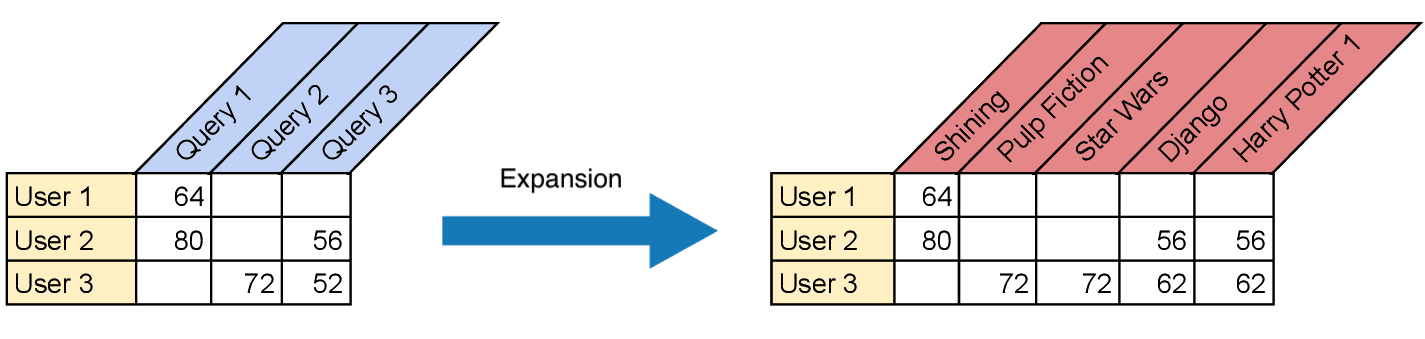
\includegraphics[width=8.5cm]{Data Mining/images/expansion.png}
\caption{Expansion Users-Queries Utility Matrix into Partial Users-Items Utility Matrix}
\label{fig:expansion}
\end{figure}

\subsubsection{Item-Item collaborative filtering execution on the users-
items utility matrix}
\label{sec:expanded-cf}
In this step, the main objective regards filling the \textit{users-item\_utility\_matrix} previously computed in order to obtain a complete matrix in which each row $u$ represents a user, each column $i$ represents an item and each cell ($u$,$i$) represents a rating prediction of the user $u$ for the relational item $i$.

To fill the \textit{users-item\_utility\_matrix} it was used the same \textbf{Item-Item Collaborative Filtering} approach described in the subchapter \ref{sec:compact-item-item-cf-solution}, but, instead of using the Utility Matrix $U$ as input, were used the \textit{users-item\_utility\_matrix} itself. In Figure \ref{fig:item-ritem-cf} it is shown an example of the result obtained by doing so.

\begin{figure}[h!]
\centering
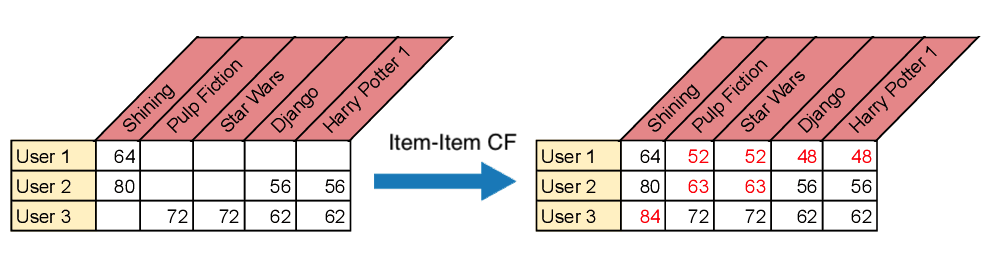
\includegraphics[width=8.5cm]{Data Mining/images/item-ritem-cf.png}
\caption{Item-Item Collaborative Filtering applied on the Expanded Utility Matrix}
\label{fig:item-ritem-cf}
\end{figure}

\subsubsection{Compression users-items to users-queries utility matrix} \label{ch:4.2.3}
Once the \textit{users-item\_utility\_matrix} was filled, as previously described, it was used to compute the \textit{complete users-queries\_utility\_matrix}, the requested output of the problem statement. This \textbf{compression} phase was performed by taking each user-query combination, by \textbf{identifying the items} that will be part of the result set of the query previously considered (referring to the \textit{preprocessed\_queries} matrix computed in Algorithm \ref{alg:preprocessing_queries}) and by computing the \textbf{mean} of the ratings of those items for the specific user in consideration. Those ratings are actually read from the complete \textit{users-item\_utility\_matrix} computed in the subsection \ref{sec:expanded-cf}. In order to improve both the performance in time of this compression, both its correctness, if a user-query combination was already known from the Utility Matrix $U$ given as input of the problem, those satisfaction values were also reported in the complete \textit{users-queries\_utility\_matrix} without compute any other operation. In pseudo-code, the complete \textit{users-queries\_utility\_matrix} is computed as described in Algorithm \ref{alg:reduction user-item}.

\begin{algorithm}
\caption{Complete users-queries\_utility\_matrix computation}\label{alg:reduction user-item}
\KwData{users,items,queries,utility\_matrix,users-item\_utility\_matrix,preprocessed\_queries}
\KwResult{users-queries\_utility\_matrix}

users-queries\_utility\_matrix[][] \\
\For{user \textbf{in} users}{
    \For{query \textbf{in} queries}{  
        item\_counter=0 \\
        partial\_rating=0 \\
        \uIf{utility\_matrix[user][query]==""}{
            \For{item \textbf{in} items}{    
               \uIf{preprocessed\_queries[query][item]==True}{
                    partial\_rating+= users-item\_utility\_matrix[user][item]
                    item\_counter+=1 \\
                }
            }
            users-queries\_utility\_matrix[user][query]= partial\_rating  /item\_counter \\
        }\Else{
            users-queries\_utility\_matrix[user][query]= utility\_matrix[user][query]
        }
    }
      
}
\end{algorithm}

The \textit{users-queries\_utility\_matrix} is actually complete because every user has expressed, in the \textit{users-item\_utility\_matrix}, a rating toward any item. This has as consequence that every item that compose the result of any query will be rated, and so computing the mean of those items ends up in being a trivial operation. This \textit{users-queries\_utility\_matrix}, for how it was intended during the expansion part described in the subchapter \ref{sub:expansion}, is \textbf{more reliable} in predicting the preferences regarding the queries that involves a relatively \textbf{small amount of items} in comparison to the cardinality of the entire Relational Table given as input. In Figure \ref{fig:compression} it is shown an example of the result of the compression described.

\begin{figure}[h!]
\centering
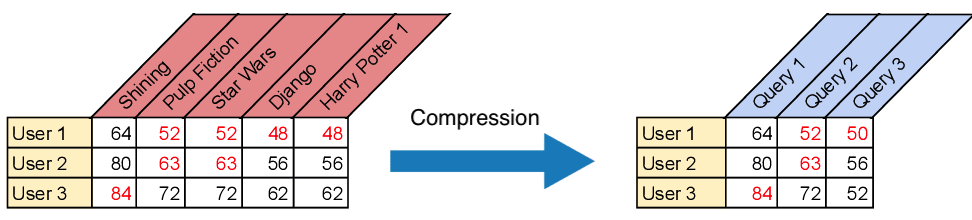
\includegraphics[width=8.5cm]{Data Mining/images/compression.png}
\caption{Compression Complete Users-Items Utility Matrix into Complete Users-Queries Utility Matrix}
\label{fig:compression}
\end{figure}

\subsection{Hybridization}
\label{cap:hybridization}
The final solution exploits the two previously computed \textit{Complete Utility Matrices} by both the \textbf{Compact Item-Item} Collaborative Filtering and \textbf{Expanded Item-Item} Collaborative Filtering components with a linear combination of their ratings driven by \textbf{query result cardinality}.
More precisely, based on the number of tuples belonging to the result set of a specific query, a different weight is assigned to the ratings of the same cell (user, query) of the two \textit{Complete Utility Matrices} to obtain a new rating.
Therefore, this rating takes into account both the rating calculated with Compact and Expanded Item-Item CF components, but with a \textbf{different weight} based on how many results are returned by the corresponding query.

In order to count the values of the result set of each query, an intermediate utility file, which is already used for the Expanded Item-Item Collaborative Filtering component and described in Section \ref{sub:expansion}, is exploited.
Leveraging the fact that each row, representing a query, acts like a BitSet of the items present in the correspondent query result set (its value is \textit{True} if the item is present), the cardinality is easily computed.
This cardinality, compared with \textbf{thresholds}, is used as discriminator for the choice of the \textbf{weights}, as illustrated in Algorithm \ref{alg:hybrid}.

There are \textbf{several ways} to assign weights and thresholds. The most accurate method of assigning them may change due to inherent hidden concepts of the particular dataset, the shape and characteristics of the dataset itself (e.g. mean, minimum, maximum of the result set cardinality). 
Each of these options needs to be carefully considered on a case-by-case basis in order to select the best way to proceed for the context being examined and finally to be able to fine-tune the parameters.

\textbf{One path} that could be chosen, that is the current one used for the evaluation experiments, consists in giving more weight to the rating provided by the \textit{Utility Matrix} of the Compact method if the query result set’s \textbf{cardinality is high}; instead, if that \textbf{cardinality is low}, a greater weight is given to the rating provided by the \textit{Utility Matrix} of the expanded method.  
Thresholds must be chosen having a clue of the mean, minimum and maximum value of the queries' result sets of the dataset analyzed, in order to achieve a \textbf{coherent splitting} of the 3 possible linear combination. For instance, if the higher threshold is set to a value higher than the widest query result set cardinality, then the first linear combination would be never used in the computation. 
For the current dataset the mean value of the result set cardinality is 221, the minimum value is 0 and the maximum value is 4696. 
Therefore the 2 threshold chosen, that are consistent with the characteristics described above, are 200 (lower bound) and 1000 (upper bound).
The three weights were chosen in such a way that the combinations did not lean too heavily toward a single approach but were \textbf{symmetrically balanced} with one another. Therefore the weights chosen and currently used are: 0.75, 0.50, 0.25 and they are used in a symmetric way as show in Algorithm \ref{alg:hybrid}.



\begin{algorithm}
\caption{Linear combination of Expanded Item-Item Collaborative Filtering and Compact Item-Item Collaborative Filtering}
\label{alg:hybrid}
\KwData{preprocessed\_queries, THRESHOLD\_1, THRESHOLD\_2, WEIGHT\_1, WEIGHT\_2, WEIGHT\_3}
\KwResult{hybrid\_utility\_matrix}
\For{query \textbf{in} queries}{

results\_in\_query[query] = \\preprocessed\_queries[query].value\_counts())

}


\For{query \textbf{in} queries}{

    \uIf{results\_in\_query[query] >= THRESHOLD\_2}{
        compact\_CF\_weight = WEIGHT\_1 
        
        expanded\_CF\_weight = 1 - WEIGHT\_1 
    }
    \uElseIf{results\_in\_query[query] < THRESHOLD\_2 \\
    \&\& results\_in\_query[query] > THRESHOLD\_1}{
        compact\_CF\_weight = WEIGHT\_2 
        
        expanded\_CF\_weight = 1 - WEIGHT\_2 
    }
    \Else{
        compact\_CF\_weight = WEIGHT\_3
        
        expanded\_CF\_weight = 1 - WEIGHT\_3 
    }

    \For{user \textbf{in} users}{
    hybrid\_utility\_matrix[user][query] = compact\_CF\_weight * compact\_CF\_utility\_matrix[user][query] + \
    expanded\_CF\_weight * expanded\_CF\_utility\_matrix[user][query]
    }
}
\end{algorithm}

The \textit{hybrid\_utility\_matrix} that can be computed with the above mentioned algorithm, is the \textit{Complete Utility Matrix} requested as \textbf{output} in the problem statement.


\subsection{Leverage the final solution to solve PART A}

The first goal met by the proposed solution is to generate a \textit{Complete Utility Matrix}. Directly related to this first objective, one can use the tool to obtain the \textit{Top-K} queries that may be of interest to the user $u$. The parameters $k$ and $u$ are therefore the input parameters of this component of the solution, referred to as \textbf{PART\_A}.

In order to perform the above described task, the user row is scanned in the \textit{Complete Utility Matrix} proposed and the \textit{Top-K} queries are given as output. The viewer can choose whether to receive only new ratings or ratings that were also previously present in the initial (sparse) \textit{Utility Matrix} $U$.


\subsection{Leverage the final solution to solve PART B}
The \textbf{PART\_B} of the project asks to develop a more general solution that is able, given some \textbf{unseen queries}, to compute a preference score about them for each user belonging to the User Set $US$ in input. Another way to interpret the task is to fill a new \textit{Utility Matrix}, so such was requested in \textbf{PART\_A}, composed by the matrix $U$ to which are appended some queries that are not rated by any users, and so that will have their corresponding column composed only by \textit{NULL} values. The solution proposed, that will be described in details in the following subchapters, use the results achieved by the PART\_A in order to compute a new \textit{users-RelationalItem\_utility\_matrix}, whose ratings are combined in order to give a prediction regarding new unseen queries.

\subsubsection{Expansion user-item}
The first operation done in order to achieve the \textbf{PART\_B} goal, as previously mentioned, is the computation of a new \textit{users-RelationalItem\_utility\_matrix}, starting from the output computed by the procedure developed in the PART\_A. This expansion follows the same underlying idea described in the subchapter \ref{sec:expansion}, even if some differences occurs due to the fact that:

\begin{itemize}
    \item The matrix used as starting point for the expansion is \textbf{complete} and so all the users will have a preference score, in the computed \textit{users-RelationalItem\_utility\_matrix}, about the same items. The score regarding the relational tuples, indeed, is retrieved by shifting the rating of a query to their results and there are not users, in the matrix obtained in PART\_A, that have rated some queries that others won't.
    \item In the expanded \textit{users-RelationalItem\_utility\_matrix} there could exists, by the way, some items that still not have a rating: it is indeed possible that some queries present in the Utility Matrix $U$, and so also in the \textit{Complete Utility Matrix} obtained from PART\_A, won't have returned some items belonging to the relational table taken into account. It is also not possible to use any collaborative filtering approach because all the users will have the cells belonging to those items \textbf{empty}. In order to fill those users-items combinations in a coherent way, it is assigned, in those cases, a score equal to the mean of the other scores expressed by the user considered for the rated relational items.
\end{itemize}
The algorithm used in order to achieve this aim is very similar to Algorithm \ref{alg:expansion-user-queries} and differs from it only for managing the previous observations, by introducing a new behavior in the case the variable \textit{denominator} will be equal to 0. The pseudocode following those steps is illustrated in Algorithm \ref{alg:partb-ch4.5.1}, where the parameter \textit{utility\_matrix} requested as input represent the \textit{Complete Utility Matrix} computed in \ref{cap:hybridization}.

\begin{algorithm}
\caption{PART\_B users-RelationalItem\_utility\_matrix computation}\label{alg:partb-ch4.5.1}
\KwData{preprocessed\_queries, users, items, queries,utility\_matrix}
\KwResult{users-RelationalItem\_utility\_matrix}
n\_results[] \\
users-RelationalItem\_utility\_matrix[][] \\
\For{query \textbf{in} queries}{
    n\_results[query] = preprocessed\_queries[query].count() \\
}
\For{user \textbf{in} users}{
     
    \For{item \textbf{in} items}{
        \For{query \textbf{in} queries}{
            \If{utility\_matrix[user][query]}{
                current\_weight=n\_results[query]
                total\_weight+=current\_weight \\
            }  
        }
        \For{query \textbf{in} queries}{
            \If{utility\_matrix[user][query]}{
                partial\_score+=utility\_matrix[user][query] * total\_weight / n\_results[query]
                denominator+=total\_weight / n\_results[query] \\
            }  
        }
        \uIf{denominator!=0}{
            users-RelationalItem\_utility\_matrix[user][item]=partial\_score / denominator \\
        } \Else{
            users-RelationalItem\_utility\_matrix[user][item]= "PLACEHOLDER"
        }
      
    }
    rating\_mean=0 \\
    item\_counter=0

    \For{item \textbf{in} items}{ \\
        \If{users-RelationalItem\_utility\_matrix[user][item]!= "PLACEHOLDER"}{\\
            rating\_mean+= users-RelationalItem\_utility\_matrix[user][item] \\
            item\_counter+=1 \\
        } \\
    }\\
    rating\_mean=rating\_mean/item\_counter\\
    \For{item \textbf{in} items}{ \\
        \If{users-RelationalItem\_utility\_matrix[user][item]== "PLACEHOLDER"}{ \\
            users-RelationalItem\_utility\_matrix[user] [item]=rating\_mean
        } \\
    } \\
} \\
\end{algorithm}

\subsubsection{Score computation}
Once that the \textit{users-RelationalItem\_utility \_matrix} is computed, it is possible, given some new unseen queries, to compute their preference scores by:
\begin{itemize}
    \item \textbf{checking} whose items of the relational table represent a result for each given query. This procedure is accomplished by executing Algorithm \ref{alg:preprocessing_queries} to which the list \textit{queries}, requested as input, represent the new queries introduced.
    \item \textbf{computing}, for each user $u$, the mean of the scores that he assigned to the relational tuples composing the results of each new query $q$ given. This result will be the one to be assigned to the cell ($u$,$q$) of the matrix in output.
\end{itemize}
The relative \textit{users-queries\_utility\_matrix}, computed by executing Algorithm \ref{alg:reduction user-item} with \textit{users-RelationalItem\_utility \_matrix} as input, will be the output requested by \textbf{PART\_B}. In order to replicate the entire procedure we will refer to Algorithm \ref{alg:preprocessing_queries} with the new queries as input, for obtaining the BitSet \textit{new\_preprocessed\_queries}, and to Algorithm \ref{alg:partb_ch4.5.2}, for getting the \textit{Complete Utility Matrix} requested by PART\_B.

\begin{algorithm}
\caption{PART\_B users-queries\_utility\_matrix computation}\label{alg:partb_ch4.5.2}
\KwData{new\_preprocessed\_queries, users, items, queries,utility\_matrix}
\KwResult{users-queries\_utility\_matrix}
users-queries\_utility\_matrix[][] \\

\For{user \textbf{in} users}{
    \For{query \textbf{in} queries}{
        partial\_query\_score=0 \\
        results\_counter=0 \\
        \For{item \textbf{in} items}{
            \If{new\_preprocessed\_queries[query][item]==True}{
                partial\_query\_score+=users-RelationalItem\_utility\_matrix[user][item]\\
                results\_counter+=1 \\
            }\\  
        }
        \uIf{results\_counter!=0}{
            users-queries\_utility\_matrix[user][queries]= partial\_query\_score / results\_counter\\
        }\Else{
            users-queries\_utility\_matrix[user][queries]=0\\
        }\\
      \\
    } \\
}
\end{algorithm}

The \textit{users-queries\_utility\_matrix}, obtained by the execution of the previous algorithms, satisfies the PART\_B of the project. Indeed, it has at each row $u$ each user presents in the user set $US$ taken as input, at each column $q$ each new queries proposed and, finally, in each cell ($u$,$q$) a prediction about the preference score of the user $u$ for the new \textbf{unseen} query $q$ based on the \textbf{users history}.





\subsection{Further improvements}

\textbf{Clustering} and dimensionality reduction techniques could improve temporal performance in the \textit{Utility Matrix}'s pre-computing phase of the current solution.
However, as stated in the introduction section of Chapter \ref{sec:solution}, the proposed solution was assumed to be in an offline context. As a result, on-demand requests for PART\_A and PART\_B tasks use pre-computed data that is saved on disk in the form of ".csv" files.

\subsection{Discarded approaches}

\subsubsection{User-User Collaborative Filtering}
The User-User Collaborative Filtering method yielded \textbf{lower performance} metrics for both the compact and expanded versions, as it can be seen is Section \ref{sec:compact-user-user-metrics}. This confirmed what was discovered in the analysis of related works in Chapter \ref{sec:related_work}: Item-Item Collaborative Filtering typically outperforms User-User Collaborative Filtering.

\subsubsection{Content-based method}

A \textbf{content-based} method was also implemented.
The initial strategy was to elect it as a method to be included in the final hybrid solution, as a weight portion, but \textbf{failed} some preliminary performance tests.

Although a fairly large number of options and alternatives were tested, good performance metrics were not obtained.

Best performances were achieved with the use of "dynamic profiles" that change based on what \textit{user-query} comparison is to be done.
Each user profile is composed of its \textit{TOP\_Q} values for each possible attribute plus the values present in the query attributes if not already present in the user profile. 




